% act_1.2
\subsection{Step reference generation}
The objective of this activity is display the UR5 robot on rviz. The simulation should start with the initial joint configuration $\begin{bmatrix} \pi & -\frac{\pi}{8} & -\frac{\pi}{6} & 0.0 & 0.0 & 0.0 \end{bmatrix}$ and then move the second and fifth joint. The joints will maintain the initial configuration during the first $2$ seconds and follow a step reference during the last $3$ seconds. The function to generate the step reference is describe in Algorithm \ref{lst:step_reference_generator} and the rosnode file to move the second and fifth joint of UR5 robot is describe in Algorithm \ref{lst:rosnode_step_reference_generator}. Finally, Figure \ref{fig:act_1.2_joint_position}-\ref{fig:act_1.2_joint_acceleration} shows the joint position, velocity and acceleration of each joint of the UR5 robot.

\begin{lstlisting}[language=Python,caption=Function to generate step reference., label={lst:step_reference_generator}]
def step_reference_generator(a):
    """
    Info: generate a constant reference.

    Inputs:
    ------
        - a: constant reference
    Outputs:
        - constant signal 
    """
    q = a       # [rad]
    dq = 0      # [rad/s]
    ddq = 0     # [rad/s^2]
    return q, dq, ddq
\end{lstlisting}



\begin{lstlisting}[language=Python, caption={Rosnode to move the second and fifth joint of UR5 robot with the requirement motion of activity 1.2.}, label={lst:step_reference_generator}]


\end{lstlisting}


\begin{figure}
    \centering
    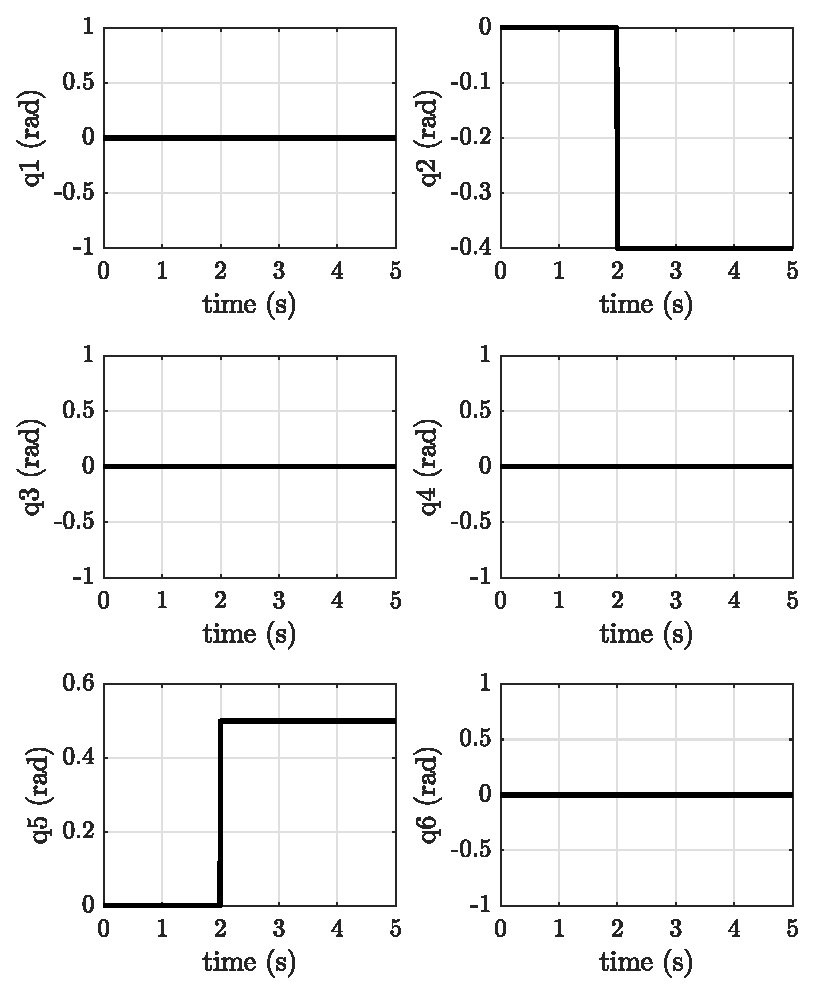
\includegraphics{images/act_1.2/joint_position.eps}
    \caption{Angular position of each joint of UR5 robot with Algorithm \ref{lst:rosnode_sine_reference_generator}.}
    \label{fig:act_1.2_joint_position}
\end{figure}

\begin{figure}
    \centering
    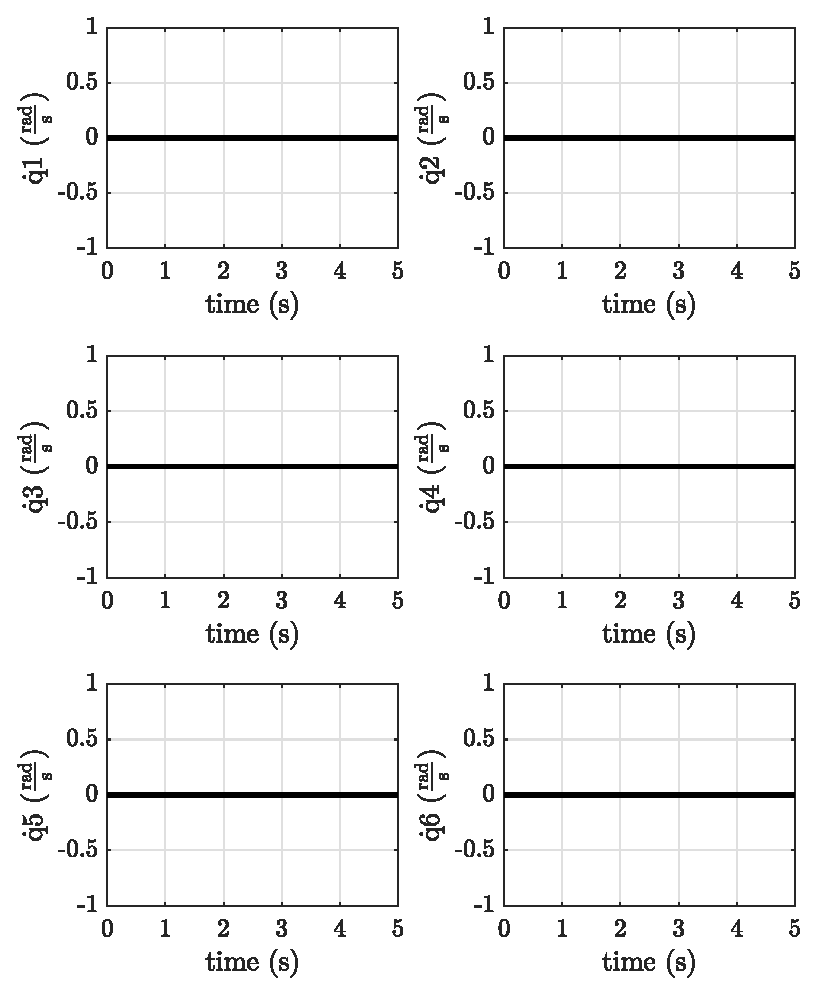
\includegraphics{images/act_1.2/joint_velocity.eps}
    \caption{Angular velocity of each joint of UR5 robot with Algorithm \ref{lst:rosnode_sine_reference_generator}.}
    \label{fig:act_1.2_joint_velocity}
\end{figure}

\begin{figure}
    \centering
    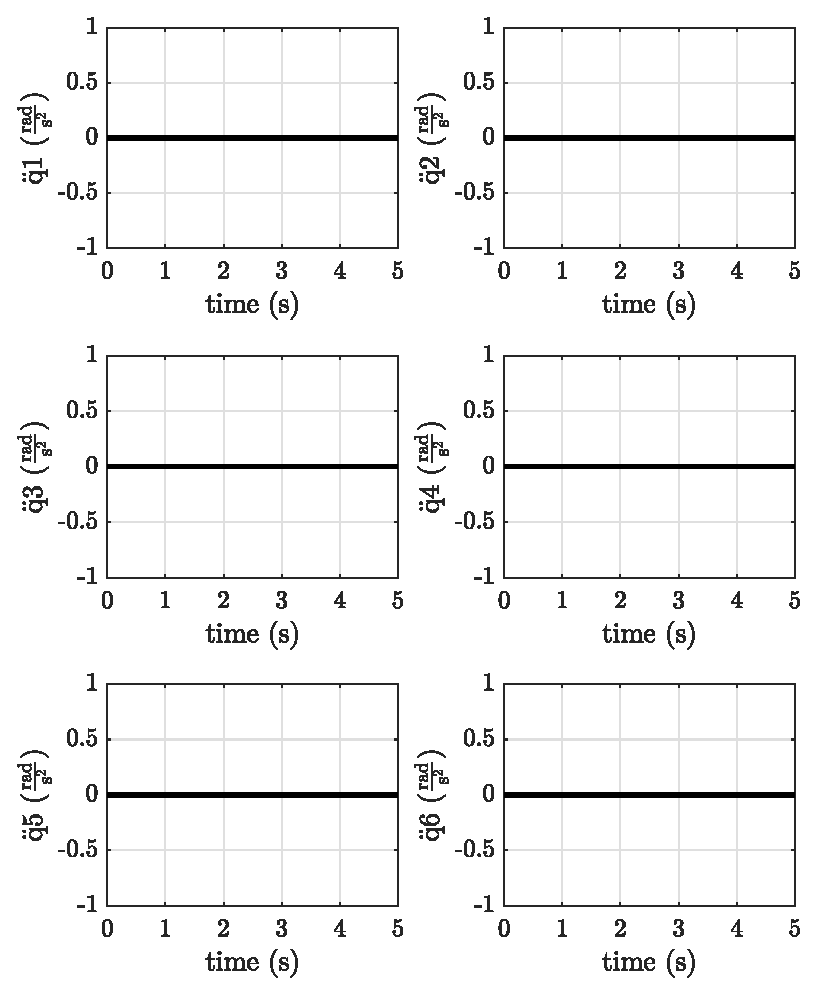
\includegraphics{images/act_1.2/joint_acceleration.eps}
    \caption{Angular acceleration of each joint of UR5 robot with Algorithm \ref{lst:rosnode_sine_reference_generator}.}
    \label{fig:act_1.2_joint_acceleration}
\end{figure}